\chapter{Implementation Test}
In this chapter, a brief demonstration testing cases are presented. To be more specifically, two testing scenarios related with \emph{CommunicationStack} applet and simulated remote server are designed. At the same time, the testing cases demonstrating communication between Smart Home web server component and Android application are designed.

\section{Remote Management Testing}
The aim of this testing scenario is to prove the feasibility of applying Smart Card and remote application/file management protocols proposed by Globalplatform to provide a secure dual authentication and messaging platform for other 
higher leveled applications. My Javacard Applet, \emph{CommunicationStack} together with correspondingly designed \emph{UTE} test cases are employed and build the testing environment.

\subsection{\emph{UTE} Test Case}

Two \emph{UTE} test cases are programmed. They are:
\begin{itemize}
\item \emph{Trigger Communication Channel with SMS}. In this test case, I simulate the open communication channel process between smart card and remote administrator server. This process is also the cornerstone for a successful remote application management.
\item \emph{Secure Messaging Exchanging} After a successful identification between communication peers and creation of communication channel, in this test scenario, smart card and remote server are going to perform secure messaging. 
\end{itemize}

\subsubsection{Trigger Communication Channel with SMS} \label{secAppletTest1}
In this test suit, UTE testing case acts as a remote administrator server and encapsulates information necessary for the construction of a secure Http channel in a \emph{TriggerPushSMS} object and sent this SMS to target smart card applet using simulated GPRS connection. The SMS structure is pictured in figure~\ref{fig:push-sms} and includes parameters which are categorized as following:
\begin{figure}[!htb]
	\centering
	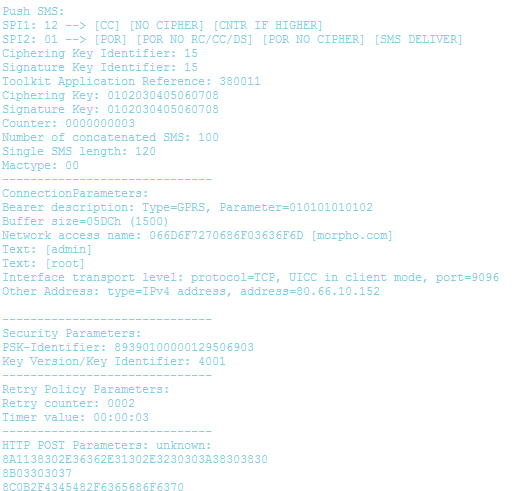
\includegraphics[width=1.0\textwidth]{Images/impl/push-sms.png}
		\caption{Push Short Message including all parameters which are necessary for the creation of communication channel}
	\label{fig:push-sms}
\end{figure}
\begin{itemize}
\item \emph{Connection Parameters}, which includes network access name, bearer description and other parameters describing the simulated remote server.
\item \emph{Security Parameters} In security parameters, proposed TLS 1.2 connection information, such as suggested cipher suit, is provided
\item \emph{Smart Card Keysets}, that consists of key identifiers as well as indicator used for the select of cipher keys and signature keys.
\item \emph{Http connection parameters}. Also parameters such as retry counter, timeout values are included in this short message.
\end{itemize}
After a successful receiving and processing of aforementioned push SMS, \emph{CommunicationStack} will preform TLS handshake with the remote server. 

The TLS \emph{client hello} is demonstrated by figure~\ref{fig:client-hello}. And in this demonstration case \emph{TLS\_PSK\_WITH\_NULL\_SHA256} is chosen. At last, the master key, shown in figure~\ref{fig:mk} is generated between remote server and card applet.

\begin{figure}[!htb]
	\centering
	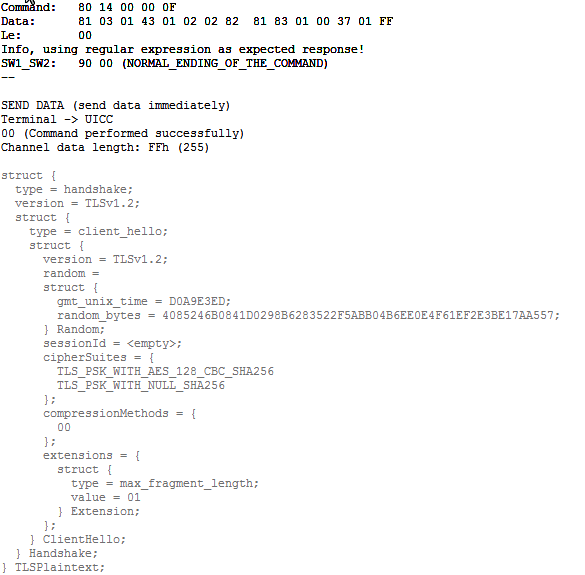
\includegraphics[width=1\textwidth]{Images/impl/client-hallo.png}
		\caption{TLS client hello sent by smart card applet}
	\label{fig:client-hello}
\end{figure}

\begin{figure}[!htb]
	\centering
	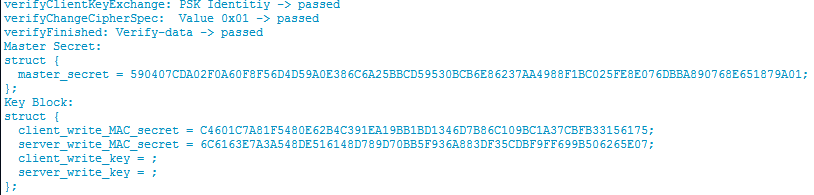
\includegraphics[width=1\textwidth]{Images/impl/master-key.png}
		\caption{Successful generation of master key between remote server and \emph{CommunicationStack} applet}
	\label{fig:mk}
\end{figure}


\subsubsection{Secure Messaging Exchanging}

\begin{figure}[!htb]
	\centering
	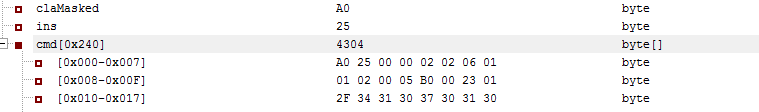
\includegraphics[width=1.2\textwidth]{Images/impl/cmd.png}
		\caption{\emph{cmd} Buffer in \emph{CommunicationStack} applet.}
	\label{fig:remote1}
\end{figure}

Based on in previous paragraph ~\ref{secAppletTest1} created secure channel and Http Connection, in this test case, smart card applet and remote server perform secure message exchange. As illustrated in figure~\ref{fig:remote1}, my applet is able to receive Http Message from remote server and retrieve the encapsulated command data. Furthermore as shown in figure~\ref{fig:remote2}, at the end of this testing scenario, remote server receives a Http message from \emph{CommunicationStack} and the content of this message is apparently secured, whose clear test is presented in figure~\ref{fig:remote2}.

\begin{figure}[!htb]
	\centering
	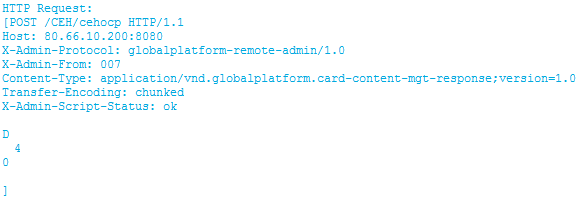
\includegraphics[width=1\textwidth]{Images/impl/http-msg.png}
		\caption{Http Response Message received by remote server}
	\label{fig:remote2}
\end{figure}

\begin{figure}[!htb]
	\centering
	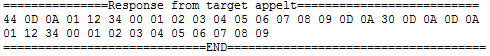
\includegraphics[width=0.85\textwidth]{Images/impl/translate.png}
		\caption{Http Content Translation}
	\label{fig:remote3}
\end{figure}

\begin{figure}[!htb]
\begin{minipage}{0.49\linewidth}
  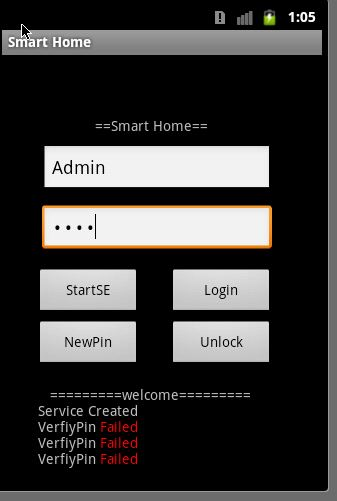
\includegraphics[width=0.8\linewidth]{Images/impl/3failed.jpg}
  \caption{Wrong PIN input}
  \label{fig:sub1}
\end{minipage}
    \hfill
\begin{minipage}{0.49\linewidth}
  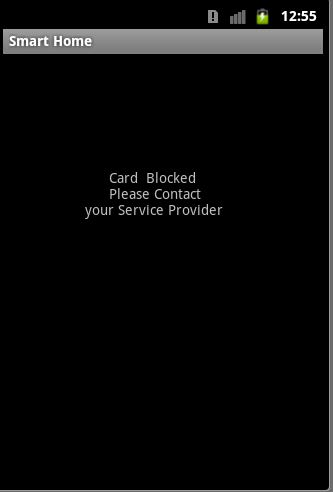
\includegraphics[width=0.8\linewidth]{Images/impl/UI3.jpg}
  \caption{PIN is blocked}
  \label{fig:sub2}
\end{minipage}
  \end{figure}
\section{Android Application Testing}
In this section, how my Android application interact with Smart Home web server and smart card applet will be demonstrated.

\subsection{PIN Verification}

As already introduced, in order to use functionalities provided by Smart Home, phone holder must authenticate himself by inputing PIN for Android application. But after three times wrong PIN input, as shown in figure~\ref{fig:sub1}, PIN will be locked. And only the service provider can unblock this PIN. 
\subsection{Communication with Web server}
After a successful identification, Android application user now can enjoy functions provided by Smart Home application, such as remote housing device management and querying historical data, as shown in following figures.

\begin{figure}[!htb]
	\centering
	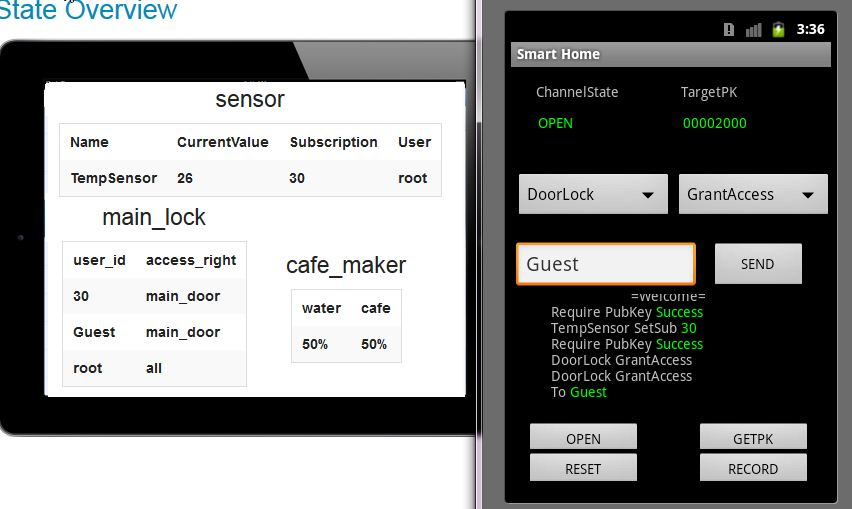
\includegraphics[width=0.85\textwidth]{Images/impl/housing-device.jpg}
		\caption{Using Android application remotely managing home devices}
	\label{fig:housing-device}
\end{figure}

\begin{figure}[!htb]
	\centering
	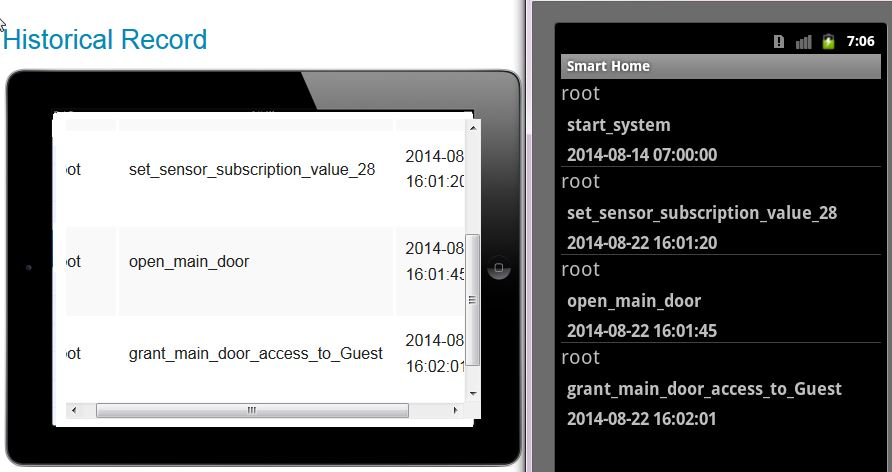
\includegraphics[width=0.85\textwidth]{Images/impl/record-query.jpg}
		\caption{Historical Record Overview}
	\label{fig:record-query}
\end{figure}
